%----------------------------------------------------------------------------------------
%	CHAPTER - INTRODUCTUION
%----------------------------------------------------------------------------------------

\chapter{Introduction} % Main chapter title

\label{ChapterIntroduction} % Change X to a consecutive number; for referencing this chapter elsewhere, use \ref{ChapterX}

%----------------------------------------------------------------------------------------
%	SECTION 1
%----------------------------------------------------------------------------------------

\section{Introduction}

With the public release of the Oculus Rift in March 2016 \citep{Oculus2016} and the HTC Vive in April 2016 \citep{Htcvive2016}, virtual reality has arrived at the consumer level and is all over the news. Although we only see the first iteration of consumer products, \cite{Gartner2015} predicts that within the next five to ten years, virtual reality will achieve mainstream adoption and enter the so called "Plateau of Producitivity". Gesture Control is even a bit ahead of VR and its mainstream adoption is already expected in the next two to five years \citep{Gartner2015}.

The focus of this thesis is on the possibilities of enhanced user interaction with virtual reality by utilizing not only hand gestures, but making use of the additional sensor information of gesture controllers and 360° motion tracking.

In the following subchapters, more background information about the topic is given as well as the definition of the problem statement. Based on this, the thesis statement is proposed and research questions are derived from. Following this, the delineations and limitations are presented before this chapter is closed with the structure of the thesis and a brief overview of the chapters and their corelations.


%----------------------------------------------------------------------------------------
%	SECTION 2
%----------------------------------------------------------------------------------------

\section{Background}

blub



(Figure \ref{fig:hypecycle}). This means that if Gartner is to be beliefed, Virtual Reality has the phase of over-excitement and unrealistic expectations already behind it and VR is close to the point where it is widely understood by the general public. A bit further than VR itself is Gesture Control that according to \cite{Gartner2015} will already reach mainstream adoption in the next two to five years.
\begin{figure}[h]
	\begin{center}
		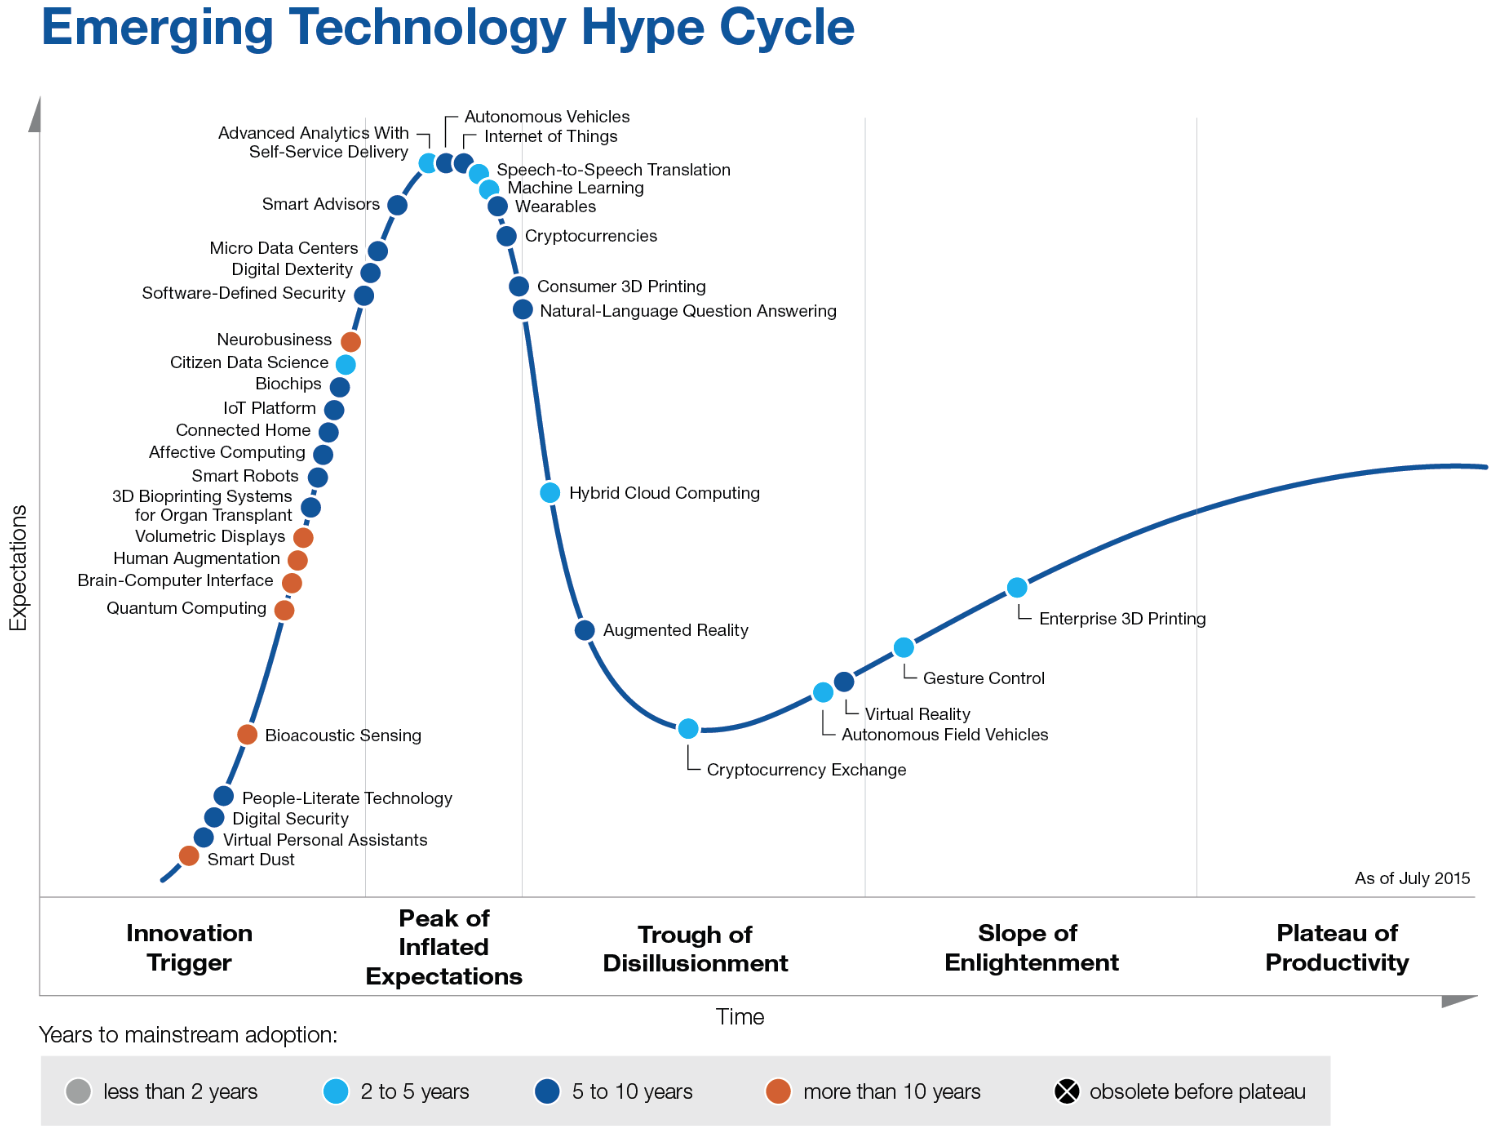
\includegraphics[width=14cm]{03_Figures/03_Gartner/Gartner_EmergingTech2015.png}
		\caption[Emerging Technology Hype Cycle]{Emerging Technology Hype Cycle \citep{Gartner2015b}}
		\label{fig:hypecycle}
	\end{center}
\end{figure}



blub
\cite{Safrudin2015}
blub

%----------------------------------------------------------------------------------------
%	SECTION 3
%----------------------------------------------------------------------------------------

\section{Problem Statement}

blub


%----------------------------------------------------------------------------------------
%	SECTION 4
%----------------------------------------------------------------------------------------

\section{Thesis Statement}

The tesis statement is as follows: \newline
\textit{The interaction with multidimensional data in virtual reality can be enhanced by utilizing gesture controllers and 360° motion tracking.}


%----------------------------------------------------------------------------------------
%	SECTION 5
%----------------------------------------------------------------------------------------

\section{Research question}

To adress the problem statement, research questions are used to break down the
In this chapter, the main research question (MRQ) as well as the sub research question (SRQ) are formulated. 
The main resarch question of this thesis is:
\textit{Can the interaction with multidimensional data in virtual reality be enhanced by utilizing gesture controllers and 360° motion tracking?}

Research questions are used to address the problem in a scientific and effective way.
Furthermore, to ask the right research questions and divide them into smaller sub research questions helps to examine the nature of the problem from different perspectives. Knowledge can be gained effectively by doing research on smaller parts – all finally contributing to the research on the given problem statement.
In this chapter two main research questions (MRQ) derived from the master thesis statement are stated. Sub research questions (SRQ) are derived from the given MRQ - supporting the research to prove that the statement is either true or not.



In this chapter the main research question (MRQ) and the sub research questions (SRQ) are formulated. The research questions guide the research. They are derived from the thesis statement. The MRQ of this thesis is:


\textit{SRQ 1: Which ways of interaction with multi-dimensional exist and what are their strengths and weaknesses?}
\newline
\textit{SRQ 2: How can retrieved sensor information be used to enhance the interaction model with multidimensional data?}



%----------------------------------------------------------------------------------------
%	SECTION 6
%----------------------------------------------------------------------------------------

\section{Research Objectives}

blub


%----------------------------------------------------------------------------------------
%	SECTION 7
%----------------------------------------------------------------------------------------

% \section{Short Overview}


%----------------------------------------------------------------------------------------
%	SECTION 8
%----------------------------------------------------------------------------------------

\section{Delineations and Limitations}

blub


%----------------------------------------------------------------------------------------
%	SECTION 9
%----------------------------------------------------------------------------------------

% \section{Underlying Assumptions}


%----------------------------------------------------------------------------------------
%	SECTION 10
%----------------------------------------------------------------------------------------

% \section{Definition of terms and concepts}


%----------------------------------------------------------------------------------------
%	SECTION 11
%----------------------------------------------------------------------------------------

% \section{Significance}


%-----------------------------------
%	SUBSECTION 1
%-----------------------------------

% \subsection{Theoretical}


%-----------------------------------
%	SUBSECTION 2
%-----------------------------------

% \subsection{Practical}


%----------------------------------------------------------------------------------------
%	SECTION 12
%----------------------------------------------------------------------------------------

\section{Thesis structure and brief chapter overviews}

blub


%----------------------------------------------------------------------------------------
%	SECTION 13
%----------------------------------------------------------------------------------------

% \section{Any other institutional requirement not covered here}



